\documentclass[aasms,12pt]{article}
\usepackage{natbib}
\setlength{\bibsep}{0pt plus 0.3ex}
\usepackage[margin=1in]{geometry}
\usepackage{sectsty}
\usepackage{graphicx}
\usepackage{hyperref}
\usepackage{epstopdf}
\usepackage{anyfontsize}
\usepackage{wrapfig}
\usepackage[skip=2pt,font=small]{caption}
\captionsetup{width=\textwidth}
\usepackage{amssymb, amsmath, amsfonts, xcolor}
\hypersetup{
    colorlinks,
    linkcolor={red!50!black},
    citecolor={blue!80!black},
    urlcolor={blue!80!black}
}


\sectionfont{\normalsize}
\subsectionfont{\small}


%\citestyle{aa}
\newcommand{\aj}{The Astronomical Journal}
\newcommand{\apj}{The Astrophysical Journal}
\newcommand{\apjl}{The Astrophysical Journal Letters}
\newcommand{\apjs}{The Astrophysical Journal Supplemental Series}
\newcommand{\aap}{Astronomy \& Astrophysics}
\newcommand{\aaps}{Astronomy \& Astrophysics Supplemental Series}
\newcommand{\mnras}{Monthly Notices of the Royal Astronomical Society}
\newcommand{\baas}{Bulletin of the American Astronomical Society}
\newcommand{\zap}{Zeitschrift für Astrophysik}
\newcommand{\sol}{\ensuremath{\odot}}
\newcommand{\RB}{Rayleigh-B\'{e}nard }
\newcommand{\grad}{\ensuremath{\nabla}}

\usepackage{fancyhdr}
\pagestyle{fancy}
\fancyhf{} % sets both header and footer to nothing
\renewcommand{\headrulewidth}{0pt}
\cfoot{\footnotesize{\thepage}}

\usepackage{titlesec}
\titleformat{\section}[hang]{\normalfont\fontsize{15pt}{18pt}\selectfont\bfseries}{\thesection}{1em}{}
\titleformat{\subsection}[runin]{\normalfont\fontsize{13.5pt}{15pt}\selectfont\bfseries}{\thesubsection}{1em}{}
\titleformat{\subsubsection}[runin]{\normalfont\normalsize\bfseries}{\thesubsubsection}{1em}{}





\begin{document}
\begin{center}
   \large\textbf{Constraining magnetic and angular momentum transport in stellar convection}\\
   \vspace{0.2cm}
   \large{Evan H. Anders}\\
   \vspace{0.2cm}
\end{center}

\vspace{-0.6cm}

\section{Motivation}

\subsection{Asteroseismology}
The advent of asteroseismic science has closely paralleled that of exoplanetary science.
The early small samples of stellar pulsations obtained by ground-based observatories \citep[e.g.,][and others]{kjeldsen&frandsen1991, bouchy&carrier2001, bedding&all2001} have given way to datasets of more than $10^4$ stars \citep[e.g.,][]{yu&all2018, santos&all2019b} in the age of CoRoT, Kepler, and K2 data.
With another 20,000 asteroseismically-interesting targets in the TESS satellite's two-year nominal mission \citep{schofield&all2019} and more interesting data from the future WFIRST and PLATO missions, it is expected that by 2030 we should have observations of $10^7$ pulsating red giants and $10^5$ dwarfs and subgiants in hand  \citep{huber&all2019}.
In addition to learning about the nature of stars aside from our Sun, asteroseismology enables us to fairly accurately determine the age of stars, thus enabling galactic archaeology, in addition to enabling us to determine the mass and radius of stars with solar-like pulsations, thus enabling the measurement of exoplanetary radii from the transit method.
Asteroseismic measurements generally rely on stellar structure models, and these models have some known deficiencies \citep{buldgen2019}, in particular their handling of complex phenomena like convection, rotation, and magnetism.
With the exponential rise in asteroseismic targets, and the projected continuation of this rise, it is crucial that the we continue to invest in the theory informing these stellar models and measurements.

The state-of-the-art method for obtaining stellar strucuture data is the use of one-dimensional models of stellar interiors from codes like MESA \citep{paxton&all2011}.
The coupling of MESA models and the GYRE code \citep{townsend&teitler2013} has enabled efficient identification of pulsational modes in a wide variety of stars.
Unfortunately, MESA models necessarily depend on one-dimensional parameterizations of convection and often employ the decades-old mixing length theory \citep[MLT,][]{bohm-vitense1958}.
MLT does an adequate job of describing convection within stars, but there are some well-known instances in which it regularly fails.
For example, 1D stellar models do not correctly produce the surface layers of stars with convective envelopes, but recent work suggests they fare better when coupled with three-dimensional surface simulations \citep{jorgensen&weiss2019}.
Furthermore, these one-dimensional models assume spherical symmetry and generally neglect the effects of rotation and magnetism.
The numerous observations of flare stars and recent asteroseismic observations which have detected magnetic field-induced frequency shifts \citep{santos&all2018} suggest that magnetism should not be neglected, and recent work shows that the specific configuration of the magnetic field impacts asteroseismic measurements \citep{thomas&all2019}.
Furthermore, it is well known that the sun exhibits differential rotation characterized by latitudinal variations in its rotational profile in the solar convection zone \citep{thompson&all1996, schou&all1998}, and differential rotation has now been observed in stars beyond the Sun \citep{benomar&all2018}.
These observations all suggest that a 1-dimensional parameterization of convection, and a neglection of complicating effects, cannot sufficiently capture the complexities of stars.
In order to properly and fully utilize the large stores of incoming asteroseismic data, we must improve the models on which asteroseismic inversions rely.

\subsection{The Solar Convective Conundrum}
The Sun is our closest star, and it is a magnetically active star.
The collection of phenomena generally referred to as solar activity, including flares and coronal mass ejections, pose a threat to our increasingly technological society.
These phenomena can wipe out power grids and harm satellites and astronauts.
Predictive power of solar phenomena has been a decades-long research goal, but will be out of reach until we have a detailed understanding of the dynamo that drives solar activity.
This dynamo is seated in the turbulent convective plasma motions of the Sun, and recent observations have called into question even our most fundamental understanding of solar convection.

Helioseismic observations by \citet{hanasoge&all2012} place an upper limit on solar convective velocity magnitudes nearly two orders of magnitude lower than those predicted by simulations or MLT.
Other helioseismic measurements using different techniques claim detections of velocity magnitudes more in line with what is expected from theory \citep{greer&all2015}, but observe an unexpected decrease in powers at large scales compared to simulations.
Even observations of convective motions at the solar surface \citep{hathaway&all2015} do not observe these anticipated, large-scale motions.
Put simply, we do not see the theorized, large-scale ``giant cells'' which would be observational manifestations of buoyant motions driven deep in the solar convection zone.
This lack of giant cells consitutes part of the Solar Convective Conundrum, and two primary hypothesis which aim to explain their absence are the ``Entropy Rain'' hypothesis and a suggestion that the solar convective interior is rotationally constrained.

The entropy rain hypothesis, first suggested by \citet{spruit1997}, suggests that downflows alone carry the solar luminosity through the solar convection zone, and has been preliminarily incorporated into a modified mixing length theory by \citet{brandenburg2016}.
Some simple simulations of \citet{kapyla&all2017} suggest that indeeed downflows may be more important than upflows in determining convective properties in stellar envelope convection.
I conducted some recent theoretical work which suggests that such a mechanism could plausibly carry the solar luminosity in the deep solar convection zone \citep{andersLB2019}.
However, most or all of the work surrounding the entropy rain hypothesis neglects magnetism and rotation.
It is unclear how these complicating effects interact with fast, small downflows like entropy rain, and it is unclear how these raindrops would alter the rotational or magnetic structure of the Sun.

Outside of the entropy rain picture, it has also been suggested that the effects of rotation alone may be sufficient to explain the solar convective conundrum.
Simulations by \citet{featherstone&hindman2016} show that as convective flows become more rotationally constrained, the spherical harmonic degree of maximum velocity power of the convection increases.
However, simulations which nominally rotate at the solar rate show \emph{anti-solar} differential rotation \citep{gastine&all2014}, and simulations at very low rossby number exhibit either differential rotation that is too-cylindrical or more reminiscent of Jupiter than the Sun \citep{brun&all2017}.
Global simulations which both suppress giant cells and correctly produce the solar differential rotation profile have not been achieved.

\subsection{Modern convective simulations}
Early simulations in stellar-like convection often focused on convection at moderate scales in Cartesian box geometries.
This work taught us a great deal about some of the complications faced by stellar convection in contained experiments.
Over the past couple of decades, these simple models have generally been replaced by either global dynamo models in spherical geometry or local Cartesian models with realistic physics.
In either case, one of the primary drivers of these simulations has been an attempt to reproduce solar or stellar observations.
This has been achieved with great success: small-scale simulations beautifully resemble magnetic sunspots to the eye, and global simulations produce cycling dynamos and differential rotations like those of the Sun.

In fact simulations of solar surface convection and even waves driven in stellar envelopes are now being used as synthetic observables and treated as true observations.
In light of our lack of understanding of the fundamentals of convection, it is important for us to step back and use simple simulations to actually understand fundamentally how stellar convection works.
Small scale simulations where vast swathes of important parameter spaces can be explored have become rare, but they can act as an important guide to large scale simulations.
DKIST!


\section{Intellectual Merit: Convection Across All Scales with Rotation and Magnetism}
\label{sct:thermals}

Stellar convection is a turbulent process, but modern computer resources cannot simulate resolved turbulent flows like those present in stars.
Moderate turbulence can be achieved in simulations either through the use of massive quantities of computational resources or through contained study of small scale dynamics.
Over the course of my postdoctoral studies, I will take advantage of the flexibility of Dedalus to study numerical simulations at three different scales, described in the following sections, in order to understand how magnetism and rotation affect convection.
In task A, I will study simulations of discrete events, or thermals \citep[as in ][]{andersLB2019}, which can allow me to study the importance of these effects on truly turbulent flows.
In task B, I will study simulations of mesoscale convection \citep[as in ][]{anders&brown2017} to gain an understanding of how these effects behave in the presence of an ensemble of convective motions, particularly at the convective-radiative interface.
In task C, I will study simulations of global stellar convection, developing an using new tools to study the importance of these effects over relaxational timescales.
These specific studies are laid out in more detail below, and each task is expected to take one full year of my three-year postdoctoral fellowship.
I will use the Dedalus pseudospectral framework \citep{burns&all2019}, which I have become proficient at using during my graduate career, to carry out these investigations.
Over the course of these three tasks, I will aim to understand two fundamental questions.
First, how do convective motions transport angular momentum and magnetic fields, and does resolving turbulent flows change this answer?
Second, how do rotation and magnetism feed back upon convective dynamics?

\subsection{Task A: Dynamics of individual downflows}
\begin{wrapfigure}{l}{0.4\textwidth}
	\begin{center}
	\vspace{-10pt}
    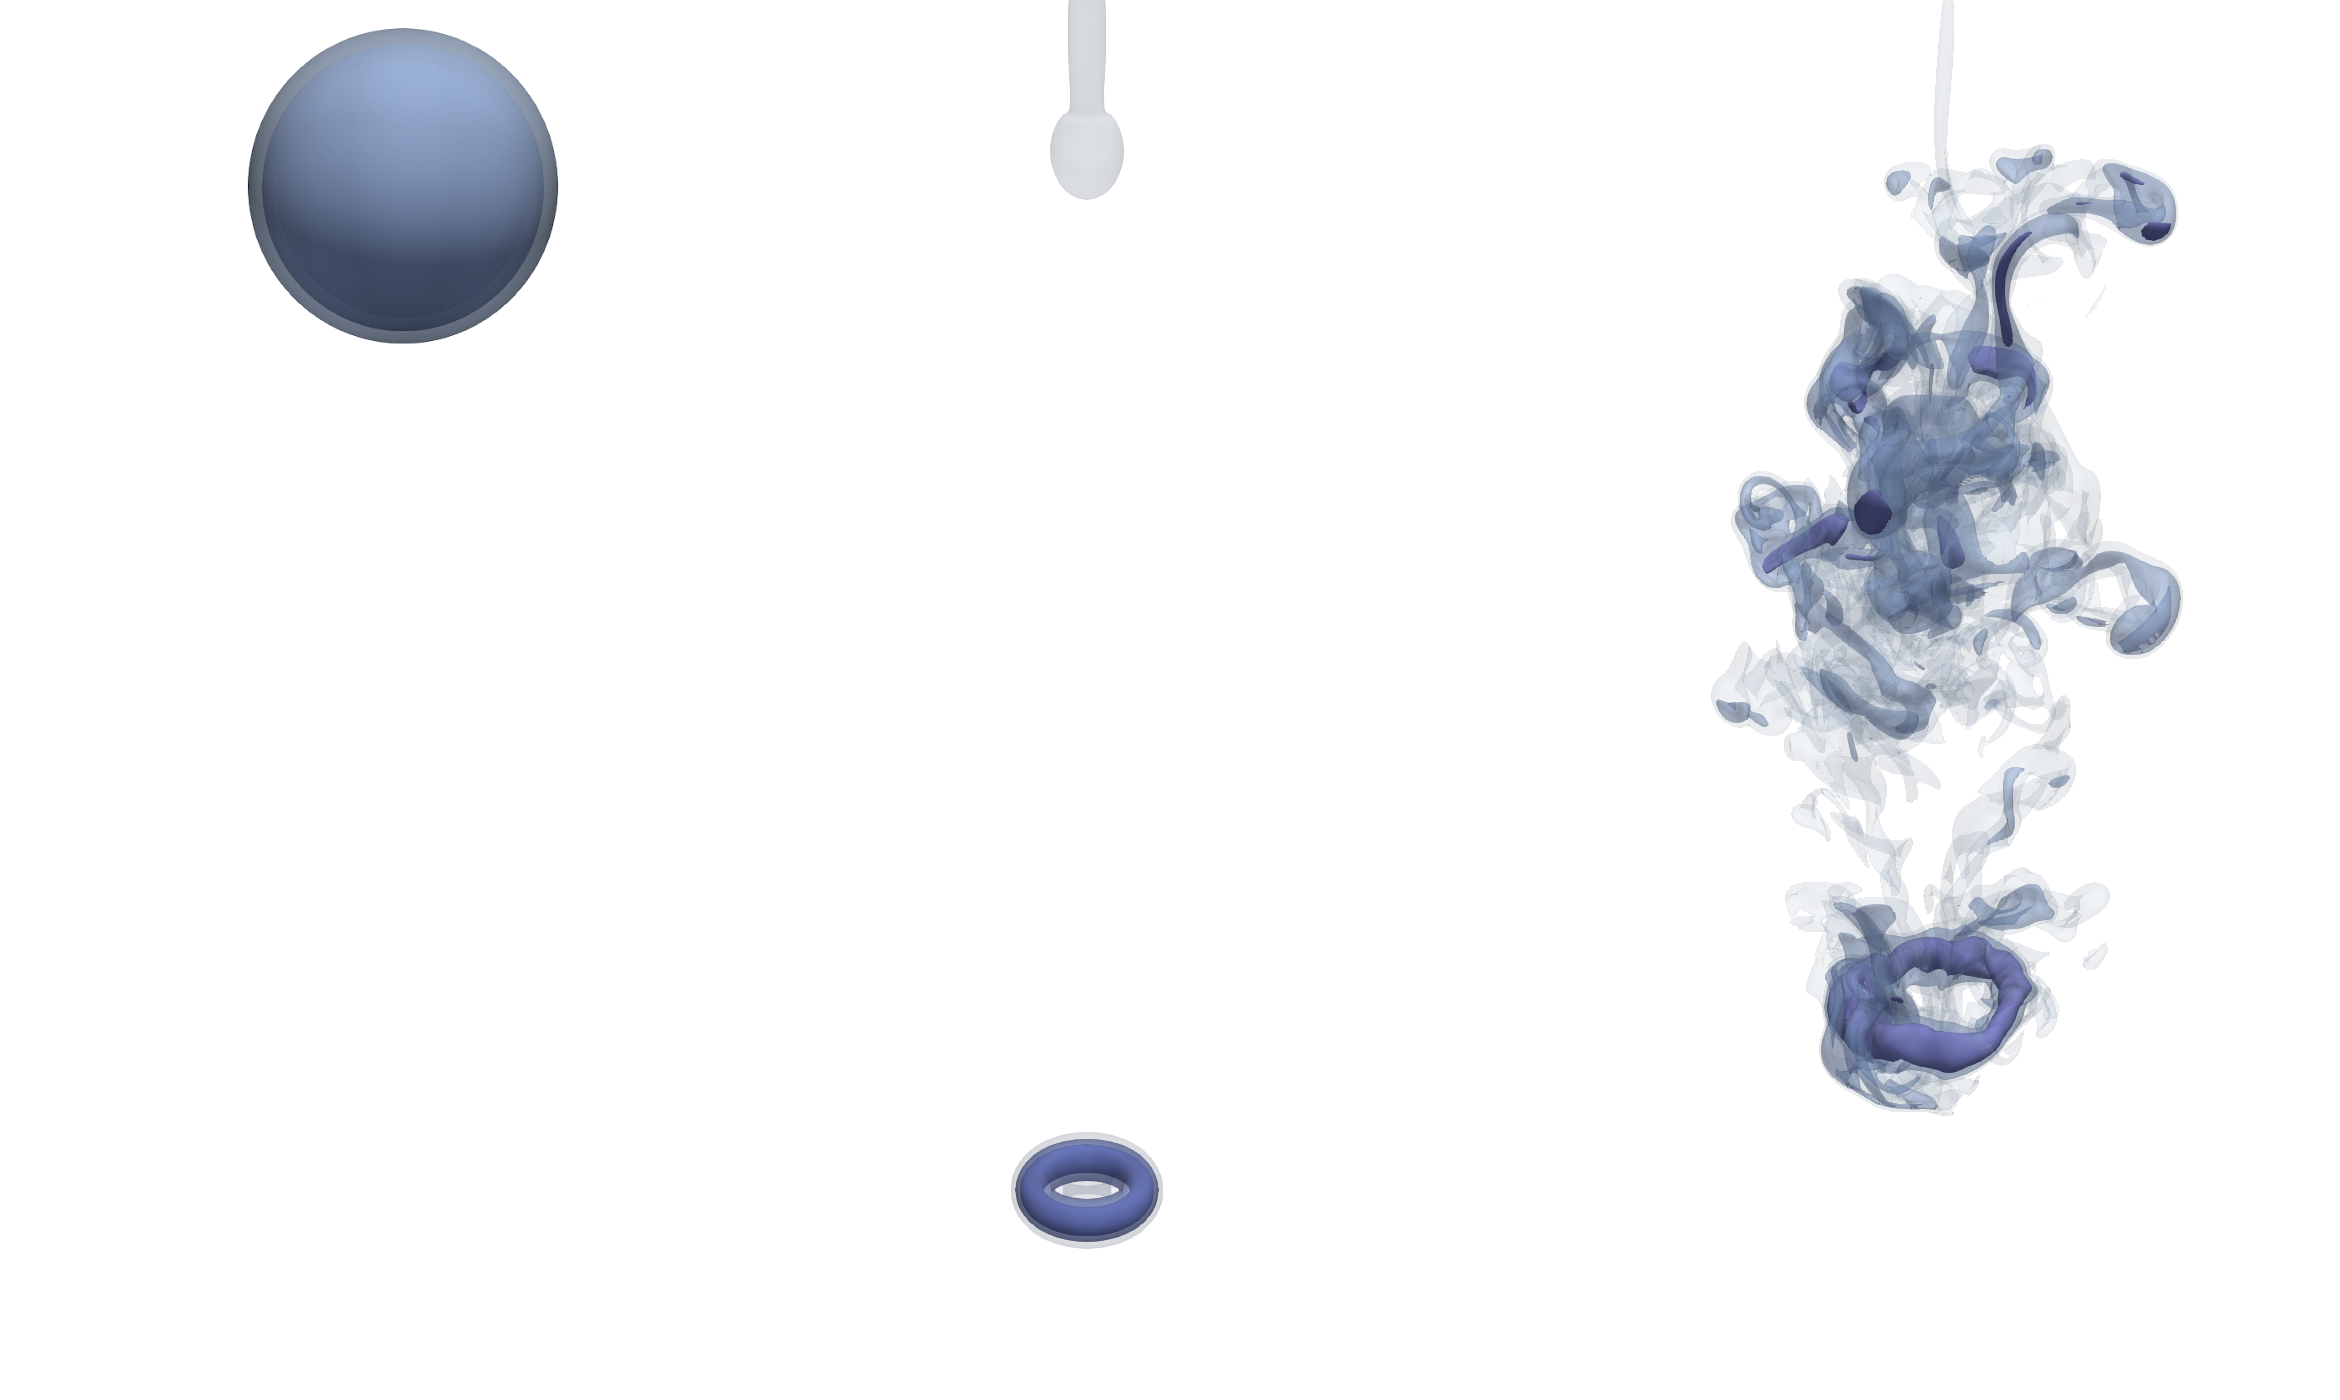
\includegraphics[width=0.38\textwidth]{./figs/thermals_comparison.png}
	\vspace{-15pt}
	\end{center}
    \caption{
	3D visualizations of the entropic signature of evolved thermals in the laminar (left) and turbulent (right) regimes.
	\label{fig:thermals_comparison} }
\end{wrapfigure}

In the envelopes of lower main sequence stars, convection occurs in the presence of extreme stratification.
Stratified convection is characterized by powerful, localized downflows, and broad, slow upflows.
Recent theory and observations (as described in section \ref{sct:convective_conundrum} suggest that downflows may be the predominant mechanism for transporting stellar luminosity in these convective zones.
Furthermore, \citet{tobias&all1998} showed that downflows in convection can effectively pump magnetic fields downwards in certain regimes.
These results suggest that downflows in stratified convection should be studied carefully so that we can better understand them; these downflows may turbulently break up into distinct pieces as they fall and these pieces can be modeled as thermals.
Thermals are regions of cold fluid which accelerate due to buoyancy forces and shape themselves into vortex rings; a visual schematic of thermal evolution is shown in Fig. \ref{fig:thermals_comparison}.
Thermals are observed and studied in the Earth's atmosphere and well understood in the Boussinesq limit.
Recently, I studied thermals as a model for solar convection and came to understand the effects of stratification on the propagation of thermals \citep{andersLB2019}.
I developed a theory for the effects of stratification and conducted high resolution simulations of thermals which verified that theory.
I now propose to extend that stratified work to further include the effects of rotation and magnetism.

Thermals provide an excellent model of stellar downflows because they are relatively easy to model analytically and to simulate.
Hydrodynamic thermals in stratified domains have a solution which is essentially fully specified by: (a) the stratification that they feel and (b) whether they are laminar or turbulent.
Thanks to my work in \citet{andersLB2019}, the influence of stratification on thermals is now understood.
During my postdoctoral studies, I will study thermals in a fixed high-stratification regime and gain a theoretical and experimental understanding of the effects of magnetism and rotation on thermal evolution.
In a purely hydrodynamical context, \citet{lecoanet&jeevanjee2019} showed that turbulence does not appreciably change the evolution of thermals.
However, turbulence creates smaller scale structures in the propagating thermals which may be important in the context of rotation or magnetism.

\subsubsection{Task A.1: Rotational filtering of downflows}
In order to study the effects of rotation, I will study thermals in simple f-plane cartesian domains.
These are plane-parallel atmospheres assumed to be at a constant latitude, and thus experiencing coriolis effects from a global rotation rate.
This complication will allow me to study the effects of rotation as a function of latitude, and in regimes where rotation is more and less important.
I propose to study thermals at three latitudes: equatorial latitudes (where gravity and rotation are perpendicular), mid-latitudes (e.g., $45^\circ$), and at polar latitudes (where gravity and rotation are parallel).
At each of these latitudes, I will study flows which experience varying degrees of rotational constraint.
I will initially study laminar thermals to understand parameter space, but will later examine select turbulent simulations in all regimes which exhibit distinctly different behavior.
The primary goal of these studies will be to determine whether downflows can be prevented from transiting convective envelopes under certain degrees of rotational constraint or at specific latitudes.

\subsubsection{Task A.2: Transport of magnetism by downflows}
I will secondarily study thermals in the presence of magnetism but absence of rotation.
The inclusion of magnetism requires a choice of initial magnetic field setup, and I will study both cases in which there is a uniform background field and where there is a thin horizontal sheet of magnetism for the thermal to pass through \citep[as in][]{tobias&all1998}.
I will vary the orientation of the initial magnetic fields and the degree of influence of magnetism on the flows, in a manner analagous to the rotational simulations in Task A.1.
These simulations will help determine how downflows may transport and generate magnetic fields, and constrain regimes in which magnetism prevents downflows from transiting convection zones. 

\subsection{Task B: Mesoscale interactions at the tachocline}
\begin{figure*}[t!]
    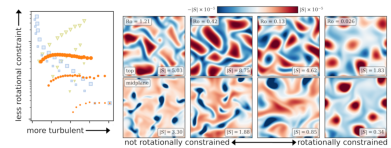
\includegraphics[width=\textwidth]{./figs/rossby_plot.png}
    \caption{(left, Fig 1b of \citet{anders&all2019}) The Rossby number, Ro, is difficult to predict as a function of the Rayleigh number, Ra, in rotating convection.
	Along traditional ``convective Rossby number'' (green) paths through parameter space, Ro increases as a function of Ra, and along constant supercriticality paths (blue) it decreases.
	Walking along paths along the newly discovered ``predictive Rossby number'' (orange) seems to hold the value of Ro, and thus the degree of rotational constraint, constant.
	(right eight panels, Fig. 2 of \citet{anders&all2019}) As you decrease the Rossby number (from left to right), traditional granular convective patterns give way to quasi-two-dimensional vortical columns of convection with very little difference between the top of the atmosphere and the atmospheric midplane (top row vs. bottom row).
	It is clear to see that changing the Rossby number strongly affects convective dynamics and therefore choosing a value of Ro that reflects the astrophysical object of interest being studied (e.g., the Sun) is crucial.
	\label{fig:rossby_plot} }
\end{figure*}

In solar-like stars, the strongly stratified convective zone overlies a stable interior radiative zone.
In the Sun, the region which separates these two zones is called the tachocline, and is characterized by both a transition from instability to stability and also strong shears as the differential rotation of the convective zone gives way to the uniformly rotating solar interior.
I will refer to the radiative-convective boundary as a ``tachocline,'' and here I propose studying convective interactions at such an interface in the absence of shear. 
Recent results suggest that convecting regions which reside above stable layers be moderately stable in the deep convecting regions.
In such regimes, downflows will be the predominant source of flux, and this begs the question: how does increased stratification, and the more intense downflows that accompany it, affect interactions at the stable interface?
Furthermore, there is a great deal of uncertainty regarding the amount of overshoot that convective motions should experience at this interface.
The magnitude of deep convective velocities and the strength of stability of the radiative zone should determine this, but deep velocity magnitudes are poorly constrained.
As a result, I propose studying how the stiffness \citep[or, whether or not convective motions can penetrate the stable region, as in][]{couston&all2017} of this interface affect the transport of angular momentum and magnetic fields into the radiative zone.

Flow balances in evolved convective dynamics are often difficult to predict from input parameters.
However, during my graduate career, I indentified and verified mechanisms for controlling the evolved Mach number \citep{anders&brown2017} and degree of rotational constraint \citep[][and Fig. \ref{fig:rossby_plot}]{anders&all2019} in mesoscale convection simulations.
The first step of Task B will use similar techniques in order to determine how to set the degree of magnetic constraint in these magnetorotational simulations.
Using that knowledge and the knowledge of task A, I will study the importance of stratifiation and stiffness of the tachocline in regimes in rotating magnetoconvection which are interesting in the stellar context.

\subsubsection{Task B.1: Controlling the importance of magnetism}
In simple models of convection, it is straightforward to control the degree of turbulence of the evolved state.
Once complicating physics are included, such as rotation and magnetism, determining the nature of evolved convective flows becomes increasingly difficult.
Interactions between boundary conditions, boundary layers, and bulk dynamics are complex and complex paths must be walked through parameter space in order to remain in specified dynamical regimes.
In \citet{anders&all2019}, I determined an appropriate path through parameter space for holding the degree of rotational constraint constant.
In this subtask, I will study nonrotational magnetoconvection and determine how to control the importance of magnetic interactions on convective flows.

\subsubsection{Task B.2: Downflow interactions at a stiff tachocline}
A strongly stratified convection zone should be characterized by intense downflows, and in this subtask I will determine how these downflows interact with different types of tachocline.
I will study very stiff tachoclines, which act similar to hard boundaries, and very soft tachoclines which convective motions can easily pass through.
\citet{tobias&all1998} showed that convective motions can effectively pump magnetic fields across soft tachoclines in certain parameter regimes.
Here I will extend that work  to determine if magnetic fields and angular momentum are capable of being pumped into stiff tachoclines by convective motions.
It is widely believed that the tachocline is a critical piece of the solar dynamo, but if convective motions are not able to pump magnetic fields into a stiff tachocline, then a different mechanism must be responsible for generating new magnetic fields.
Furthermore, a stiff tachocline could potentially insulate the solar radiative interior from convectively-driven angular momentum transport, and could explain the interior differential rotation.
These suites of simulations will test out questions like these and ask how our picture of the solar dynamo should change in the presence of a stiff tachocline.

\subsection{Task C: Global studies in relaxed atmospheres}
\label{sct:global_models}
The capstone project of my postdoctoral studies will study convection at the largest scales: global spherical simulations of rotating magnetoconvection.
The tools to perform these simulations in Dedalus already exist \citep{lecoanet&all2018} and have been tested.
One major barrier to performing global simulations is that they are costly, and some of these costs are unavoidable: highly resolved, moderately turbulent simulations necessarily take small timesteps, and therefore results come slowly.
However, some of the expense of these simulations is often time wasted waiting for the atmospheric structure and mean flows to converge to an equilibrium state.
For example, the thermal structure of the Sun is thought to evolve over its Kelvin-Helmholtz timescale of $10^7$ years, which is significantly longer than its convective overturn time of five minutes at the solar surface, although still much shorter than its main sequence lifetime.
As simulations approach the parameter regime of stars, relaxation and dynamical timescales become extremely disparate, and in general numericists must choose between having state-of-the-art turbulence or converged, statistically equilibrium dynamics -- but not both.
During this third task, I will develop, test, and utilize a community tool which effectively establishes mean flows and evolves atmospheric structures by taking much larger timesteps than those of convection.
By doing so, I will enable global dynamo simulations which are both relaxed and exhibiting state-of-the-art turbulence.

During my graduate career, I studied a mechanism for accelerating the long thermal relaxation timescale in convective systems \citep{anders&all2018}.
In this work, we discovered that a tool like the one I am proposing here can be feasibly implemented and tested for accuracy, albeit we previously studied this in a very simple system.
While studying moderately turbulent flows, we found that our tool reached a relaxed state using an order of magnitude fewer computational resources than when waiting for a standard thermal relaxation timescale.
These speedups make achieving thermal relaxation in state-of-the-art simulations feasible.

\subsubsection{Task C.1: Accelerated evolution of global simulations}
During my postdoctoral studies, I will extend my accelerated evolution method to the evolution of thermodynamic and angular momentum profiles in global simulations.
The development of this extension will be grounded in understandings gained in tasks A and B.
In particular, task A will inform which terms in the equations importantly adjust the mean field in certain regimes, and task B will inform how to implement this technique near tachocline-like interfaces.
As I did in \citet{anders&all2018}, I will verify that this method produces the same results as a long relaxation in modest parameter regimes to build trust in the method.
Once developed, this tool will be made publicly available (as described in the part of the proposal where I describe these things).

\subsubsection{Task C.2: Relaxed simulations of the solar dynamo}
I will study simulations of the interior solar convection zone in regimes where flows feel the effects of both rotation and magnetism, using the knowledge from task B to determine how to set up such simulations.
Using the tool developed in task C.1, I will accelerate the evolution of these simulations.
Then, using relaxed atmospheric structures and mean flows, I will study the time-dependent nature of the magnetic field evolution.
In most modern dynamo simulations, the evolution of magnetic fields are measured during the relaxation process, and it is possible that the time-dependent dynamo behavior of the simulation is strongly influenced by the underlying evolution of the mean state.

While these simulations will be largely targeted in the solar context, the accelerated evolution tools which will be developed and tested here could have great benefits for asteroseismic research.
Recently, \citet{jorgensen&weiss2019} coupled three-dimensional, global simulations with 1-dimensional stellar structure tools in order to more accurately produce stellar structure profiles to great success.
The fast equilibration of angular momentum and thermal profiles described here is essentially equivalent to taking timesteps which superstep the convective motions, similar to those taken in any one-dimensional stellar structure model.
Put simply, these accelerated evolution techniques would be a first step to enabling the coupling of 1-dimensional stellar structure codes with realistic statistics from converged global convection.
Future asteroseismic inversions will then benefit from stellar structure models which are influenced by three-dimensional convection including complicating effects like magnetism and rotation.

\subsection{Computational Feasibility}
Tasks A-C are arranged logically from smallest to largest scales, but this also parallels the fact that they will range from least to most expensive.
Based on the work in \citet{anders&brown2017, anders&all2018, anders&all2019, andersLB2019}, Dedalus takes $\mathcal{O}(10^3)$ cpu-sec per iteration for a run with a grid resolution of 384$^3$ on a system comparable to NASA Pleiades.
Task A runs of thermals will take $\mathcal{O}(10^4)$ iterations each, while turbulent runs in tasks B and C will take $\mathcal{O}(10^6)$ iterations each.
Laminar thermal simulations thus cost roughly 5000 cpu-hours each, while turbulent thermals cost roughly $10^6$ cpu-hours each.
State-of-the-art simulations in tasks B and C will cost roughly $10^6$ cpu-hours each.
The projects described here total 5-10 million cpu-hours per year in tasks B and C, with less (2-3 million cpu-hours) in the first year while thermals are being studied.

The computational cost of task A should be feasible to obtain on Northwestern's 11,800-core Quest supercomputer.
In order to increase my access to computational resources and to allow for larger scale runs in tasks B and C, I will leverage my AAPF fellowship and apply for time on NSF XSEDE resources such as Stampede2, Comet, or Bridges.




\section{Collaborative studies at CIERA}
\label{sct:northwestern}
Northwestern university, and specifically the CIERA institue, is the perfect location for me to carry out the work proposed here.
Dr. Daniel Lecoanet, who will be my primary advisor and collaborator, will be arriving in the Fall of 2020, and I would be arriving concurrently.
As one of the code's founders, Dr. Lecoanet an expert in Dedalus and his past work on thermals \citep{lecoanet&jeevanjee2019, tarshis&all2018}, convection \citep{lecoanet&quataert2013, lecoanet&all2014, couston&all2017}, rotating convection \citep{couston&all2019}, and global simulations \citep{lecoanet&all2018} make him excellently qualified to advise me on the projects proposed here.
Furthermore, I have already published one paper in collaboration with Dr. Lecoanet and so there would be no lag in figuring out a successful collaborative and professional relationship upon my arrival.
In addition to Dr. Lecoanet, Dr. Yoram Lithwick would be an excellent partner for collaboration due to his past work on rotating convection \citep{BDLithwick2014} and his continuing collaborations on studying careful and numerical problems in fluid disks \citep{LDLithwick2019} and planetary systems \citep{hadden&lithwick2018} would provide excellent opportunities for collaboration.
Despite working on disparate applications, I also anticipate that the work proposed here will benefit from fruitful conversations with other members of the institute, such as Dr. Sasha Tchekhovskoy, whose background in general relativistic MHD simulations is extensive \citep[as in e.g.,][]{tchekhovskoy&bromberg2016}.

Furthermore, in addition to the focused educational and outreach projects below, being centered at CIERA will provide me with numerous small scale opportunities to participate in public outreach.
CIERA's Astronomy on Tap program as well as its CIERA Astronomer Evenings provide bite-sized and accessible ways to interact with the public.
Dearborn Observatory's observation tours are very similar to the public open houses I helped host at CU Boulder's Sommers-Bausch observatory.
The state-of-the-art Adler planetarium also provides similar opportunities such as its \emph{`Scopes in the City} program or its Space Visualization Lab astronomy conversations.


\section{Broader Impacts: Supporting the growth of young career scientists as educators and individuals}
\label{sct:outreach}
Through the implementation of two small programs which leverage collaborations with existing programs or institutes at Northwestern, I aim to support diverse young career students at the university level with a network of supportive peers while also creating meaningful opportunities for them to develop as educators and professionals.
Their development will also result in the teaching of authentic inquiry at the high school level, thereby serving the broader community.

Side note: NSF language that is applicable and that I need to work in here: ``Such outcomes include, but are not limited to: full participation of women, persons with disabilities, and underrepresented minorities in science, technology, engineering, and mathematics (STEM); improved STEM education and educator development at any level; increased public scientific literacy and public engagement with science and technology; ...development of a diverse, globally competitive STEM workforce...''



\subsection{Teaching/Outreach: Developing early career scientists as teachers}
During my graduate career I twice participated in the University of California Santa Cruz's Institute for Scientist and Engineering Educators Professional Development Program (UCSC ISEE PDP), an NSF-funded program which teaches early career scientists the basics of teaching pedagogy in the context of developing and teaching an authentic STEM inquiry activity.
While the PDP is open to graduate students, postdocs, and faculty members at all universities in the US, in general only a small group of individuals from any one institution can participate in a given year.
My experiences in this program helped me gain confidence in knowing that teaching is an important piece of my future career, and laid the foundation of my knowledge of what it means to be a teacher and how teaching can be informed by scientific literature.
I propose to develop a one-semester course for graduate students and senior undergraduate students which teaches the basics of teaching pedagogy and culminates in authentic teaching experiences in either high school classrooms.
I will spend 10-15\% of my time during my first year as a postdoctoral researcher developing and establishing the infrastructure for this course, then I plan to teach the course in the Fall of 2021 and 2022.
Over the course of Spring and Summer I will iterate and improve on my course materials based on student performance and feedback, and in Spring and Summer of 2023 I will ensure that the course materials are made available to Northwestern faculty before my fellowship ends.

The culminating project of this course will be an authentic teaching experience for the students, something which many young scientists do not have in their undergraduate or graduate preparation.
In order to coordinate these teaching experiences, I will leverage connections with the CIERA-based and NSF-funded \href{http://gk12.ciera.northwestern.edu/}{Reach for the Stars} program, a GK-12 program.
Reach for the Stars is a selective program which offers a small number of graduate students an opportunity to spend 10-15 hours per week in the high school classroom leading young students through authentic scientific inquiry experiences while teaching those students how to think computationally and use computational tools.
Exposing young students to authentic scientific inquiry activities is crucial because students not only learn STEM content but also participate in using STEM practices, such as creating hypotheses or designing and carrying out investigations.
Reach for the Stars' \href{https://avault.github.io/}{Vault} program does an excellent job of providing a space for students to participate in these practices.
These practices are often not explicitly taught, and this can make it difficult for scientists to communicate their processes.
Fortunately modern literature \citep[e.g.,][]{dasgupta&all2014} is breaking down struggles that students face in learning the \emph{practices} of science, which can help guide our design of in-the-classroom activities which focus on teaching these practices.
This class will complement Reach for the Stars by providing an opportunity for professional development to a larger number of students which is overall a smaller time commitment and less selective while still offering the students an opportunity for professional growth and impactful outreach.

One guiding principle of proper course design is backwards design \citep{wiggins&mctighe1998}, which is \emph{logically} foward, but \emph{in practice} backwards from how many courses are designed.
In essence backward design states that you start with the learning outcomes you want your students to achieve, then you design careful assessments to determine whether or not those learning goals were met, and \emph{only then} do you design the course content.
An understanding of the backwards design process is one of the learning goals I have for students who take this course, but I will also use these principles in the design of this course.
Since the culminating project of the course for the students will be to teach a topic in the high school classroom, I will rely on the high school teachers to provide us with a learning outcome that fits their curriculum, and it will then be the role of the students to work backwards from that goal in the design of their inquiry activity.

I will design specific tasks that students will undergo during Fall 2020 - Spring 2021, but in general the course will cover four broad topics, each of which has been heavily influenced by the groundwork and structure of ISEE's PDP program.
In the first unit, students will learn about backwards design in the context of inquiry activities, including specific care about how to set both content and practice learning goals for their students and different activity structures which leave space for authentic inquiry while also ensuring students arrive at those learning outcomes.
In the second unit, we will discuss different types of assessments, when these types of assessments are appropriate, how to create honest and fair rubrics, and how to align a rubric with an assessment.
In the third unit, we will discuss equity and inclusion, including published research regarding the effects that inequities have on students, and discuss how to design inclusive activities with multiple pathways for success so that all learners can achieve the learning goals.
In the fourst unit, students will experience the culmination of the work that they have done through the semester by teaching in the college classroom, and then we will discuss methods for iterating on course design in order to improve it for the future.

This course will provide young career scientists with a foundation in how to teach, things to consider while teaching, and will also give them an opportunity to try out some teaching practices in a fairly low-stakes setting.
The students will be graded on their thoughtful creation, analysis, and reflection on their course design rather than on the specific teaching outcomes of their activity.
Furthermore, the culminating project for each group of students is by definition an outreach activity: the students will go into nearby high school classrooms, engage with young students about science, provide authentic and inclusive experiences in STEM, and in doing so broadly impact the nearby community.

\subsection{Inreach: Undergraduate and graduate peer mentorship}
The path to a career in the US STEM workforce is a leaky pipeline.
Data show that in particular, underrepresented minority groups and women pursue careers in STEM fields at a rate which is disproportionately low compared to the share of the total population that those groups constitute \citep{corbett&hill2015, nsf2019}.
While a great deal of focus is rightly placed on changing the career outlooks of these groups before the collegiate level, the pipeline continues to leak at the baccalaureate and post-baccalaureate levels, and underrepresentation becomes more severe.

Mentoring has long been known to play a significant role in increasing retention and helping new departmental members acclimate to the department climate \citep{hunt&michael1983}.
Establishing robust mentoring programs based on evidence and knowledge of the recent literature in mentorship \citep[as in e.g.,][]{crisp&all2009, crisp&all2017} can be one critical component of helping broaden participation of underrepresented and marginalized groups in the STEM workforce.
During my graduate studies, I spent three years working with the University of Colorado's CU-STARs group.
CU-STARs is a combined ``outreach'' and ``inreach'' program with the dual aims of increasing STEM engagement for students at underserved, rural schools across Colorado while decreasing attrition of underrepresented groups in CU Boulder's Astrophysical and Planetary Sciences department.
One of my many roles as a graduate student administrator in this group was to mentor undergraduate students, although we were never formally trained in mentoring, nor did we have a robust mentoring structure in place to support mentors and mentees alike.

During my years at Northwestern, I propose to work with the experts in Northwestern's \href{https://www.northwestern.edu/searle/index.html}{Searle Center for Advanced Teaching and Learning} to develop peer mentoring programs within Northwestern University's applied math department and the department of physics and astrophysics.
The goal of this program will be to connect students with peers who are slightly more advanced in their careers.
For example, entering undergraduate mentees would connect with junior or senior undergraduates in the field; senior undergraduates mentees could connect with young graduate student mentors; young graduate student mentees could connect with senior graduate students; and senior graduate students could connect with postdoctoral students.
In general, we would aim to connect young scientists who are still at a close enough level of their career to fully understand the experiences of one another to give young students advice and provide them with a professional support network.

I will lay the groundwork for this organization in my first year at Northwestern and plan to roll it out in my second year, starting in the fall of 2021.
My first year will be spent collaborating with my hosting department, as well as other very related departments like the department of Physics and Astronomy, in order to gain university buy-in at the faculty level to ensure that this program will continue to run after I leave.
I will also collaborate with the Searle Center and others to ensure that I establish proper training for mentees.
Furthermore, I will begin searching at the University level for sustainable \href{https://www.northwestern.edu/studentorgs/org-officers/funding/index.html}{funding} so that this organization can support the purchasing of coffee for mentor meetings.
I will also aim to secure enough funding for the organization to buy snacks for infrequent social meetings.

\subsection{Personal career growth and development}
Need to write this in more words, but basically my past experiences have shown me that I truly enjoy both research and teaching.
Setting up these programs will allow me to grow in the teaching / service aspect of an academic career while also giving younger students a taste of that aspect of this career path so that they can help decide if they like it.



\section{Summary and Perspectives}
\label{sct:summary}
TODO

\bibliographystyle{apj}
\bibliography{biblio}
\end{document}
